\subsection{Erstellung des RPi-HATs}\label{hw_hat}
Zur Schaltplanzeichnung haben wir das OpenSource-Programm KiCAD genutzt.
Dieses ist für zahlreiche Betriebssysteme verfügbar.\footnote{Siehe \url{https://www.kicad.org/download/}} 
Teilebibliotheken sind zahlreich im Internet verfügbar, wir haben uns auf den Anbieter SnapEDA beschränkt, da dieser die meisten gängigen Bauteile für Elektronik-CAD-Systeme anbietet. 
Eine weitere Bezugsquelle ist der Verkäufer Digi-Key Electronics, der einen Großteil seines Sortiments an SMD-Bauteilen als Bibliothek anbietet\footnote{Siehe \url{https://www.digikey.de/de/resources/design-tools/kicad}}. 
Als Grundlage für den HAT sollte die Projektvorlage ,,Raspberry Pi - 40-Pin HAT'' von Jon Buford dienen.
Diese Vorlage richtete sich nach den offiziellen HAT-Spezifikationen für den Raspberry Pi\footnote{Siehe \url{https://github.com/raspberrypi/hats}}.\par
\noindent Zu Beginn des Projekts haben wir in KiCAD die GPIO-Ports anhand der offiziellen Dokumentation beschriftet, um das Nachschlagen der Belegung in Zukunft zu vermeiden.
\begin{figure}[H]
	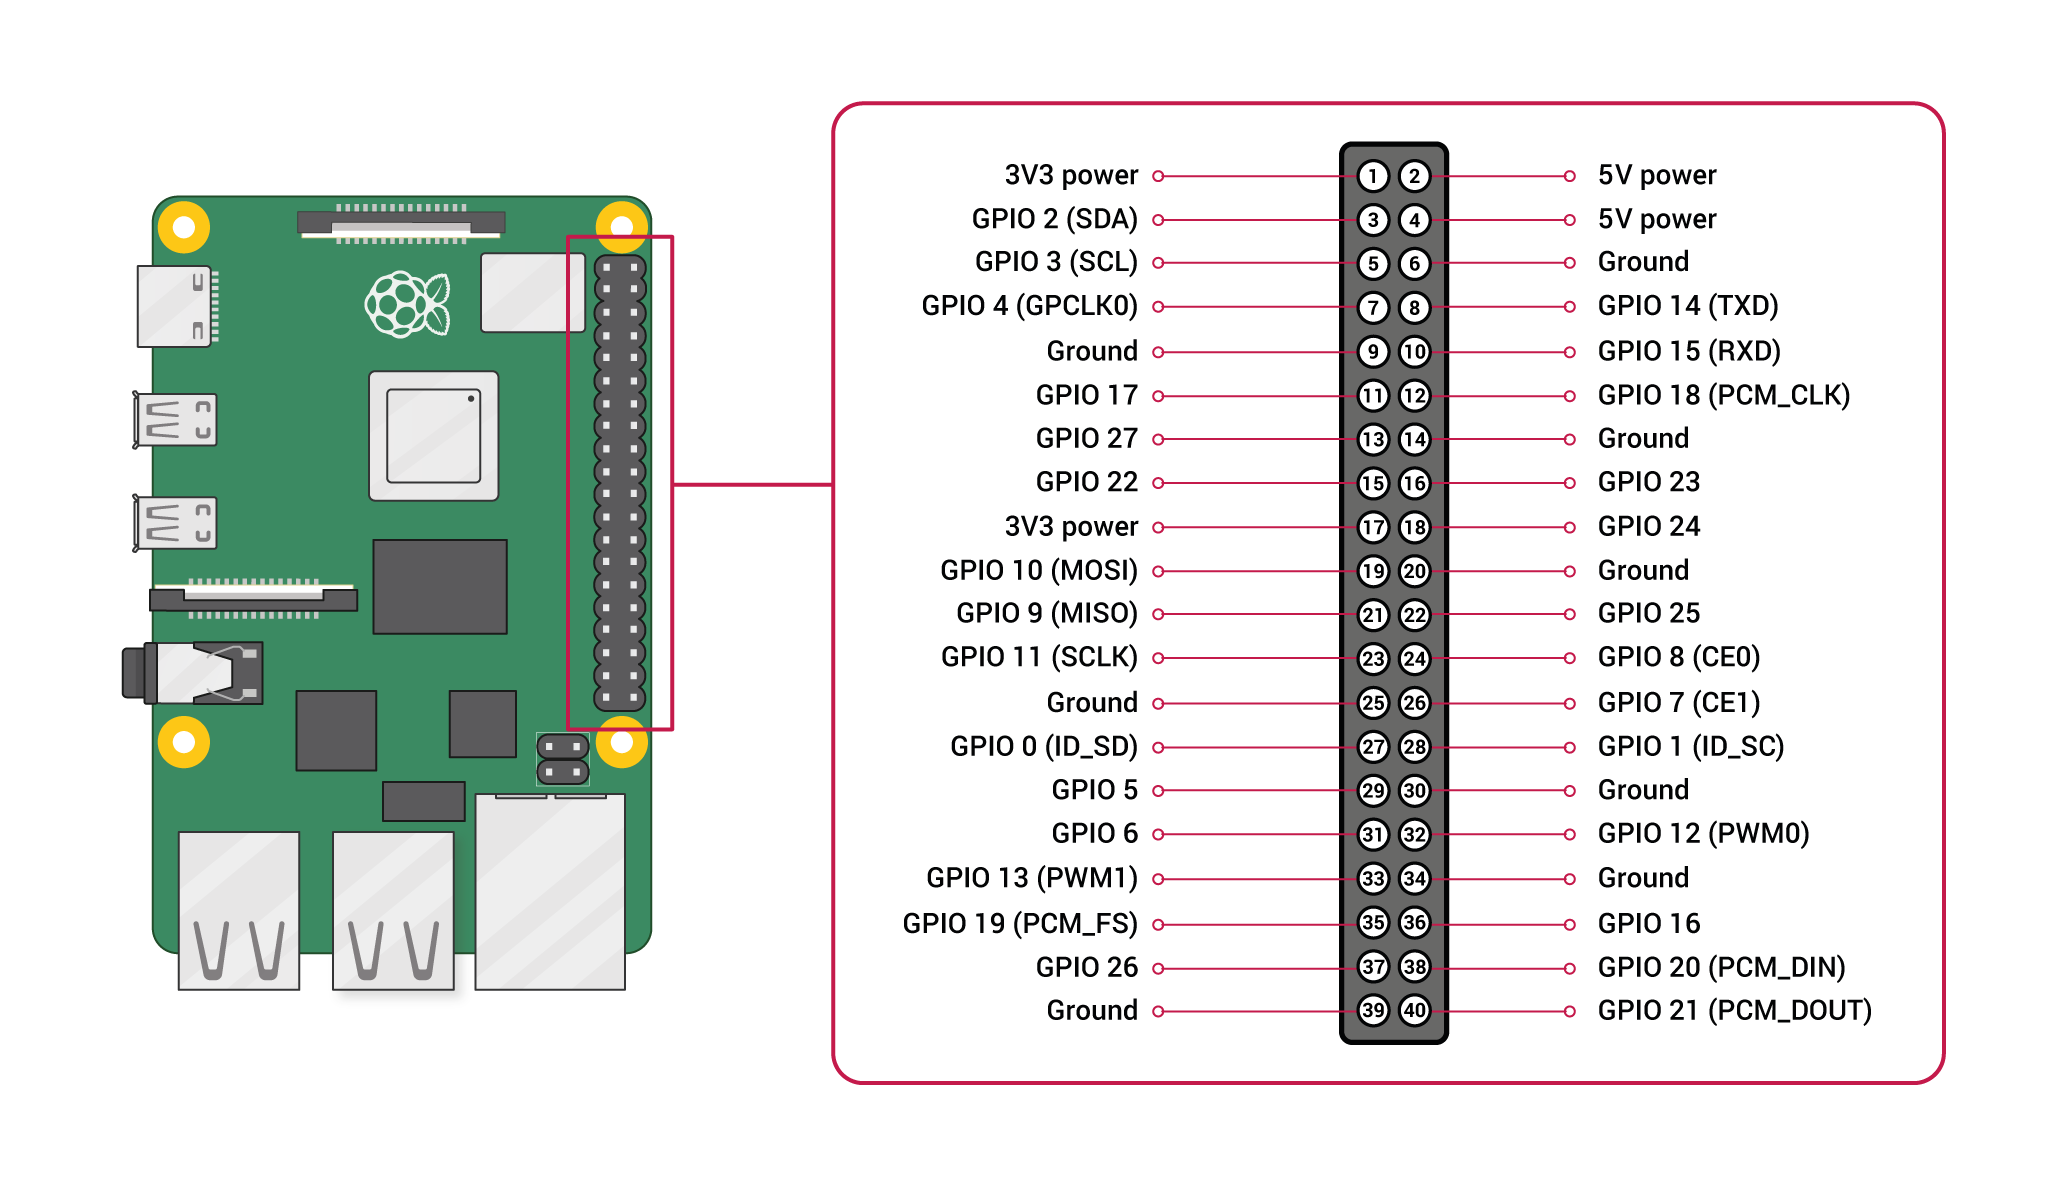
\includegraphics[width=1\textwidth]{img/GPIO-Pinout-Diagram-2.png}
	\caption[Raspberry Pi 4 GPIO-Pins]{Raspberry Pi 4 GPIO-Pins}
	\label{rpi-gpio-pins}
\end{figure}
\par
\noindent Anschließend haben wir die (unserer Meinung nach) benötigten Komponenten auf den Schaltplan gezogen beziehungsweise vorher importiert und dann versucht, diese sauber zu verdrahten (vgl. Abb. \ref{hat-design}: \nameref{hat-design}.\par
\begin{figure}[H]
	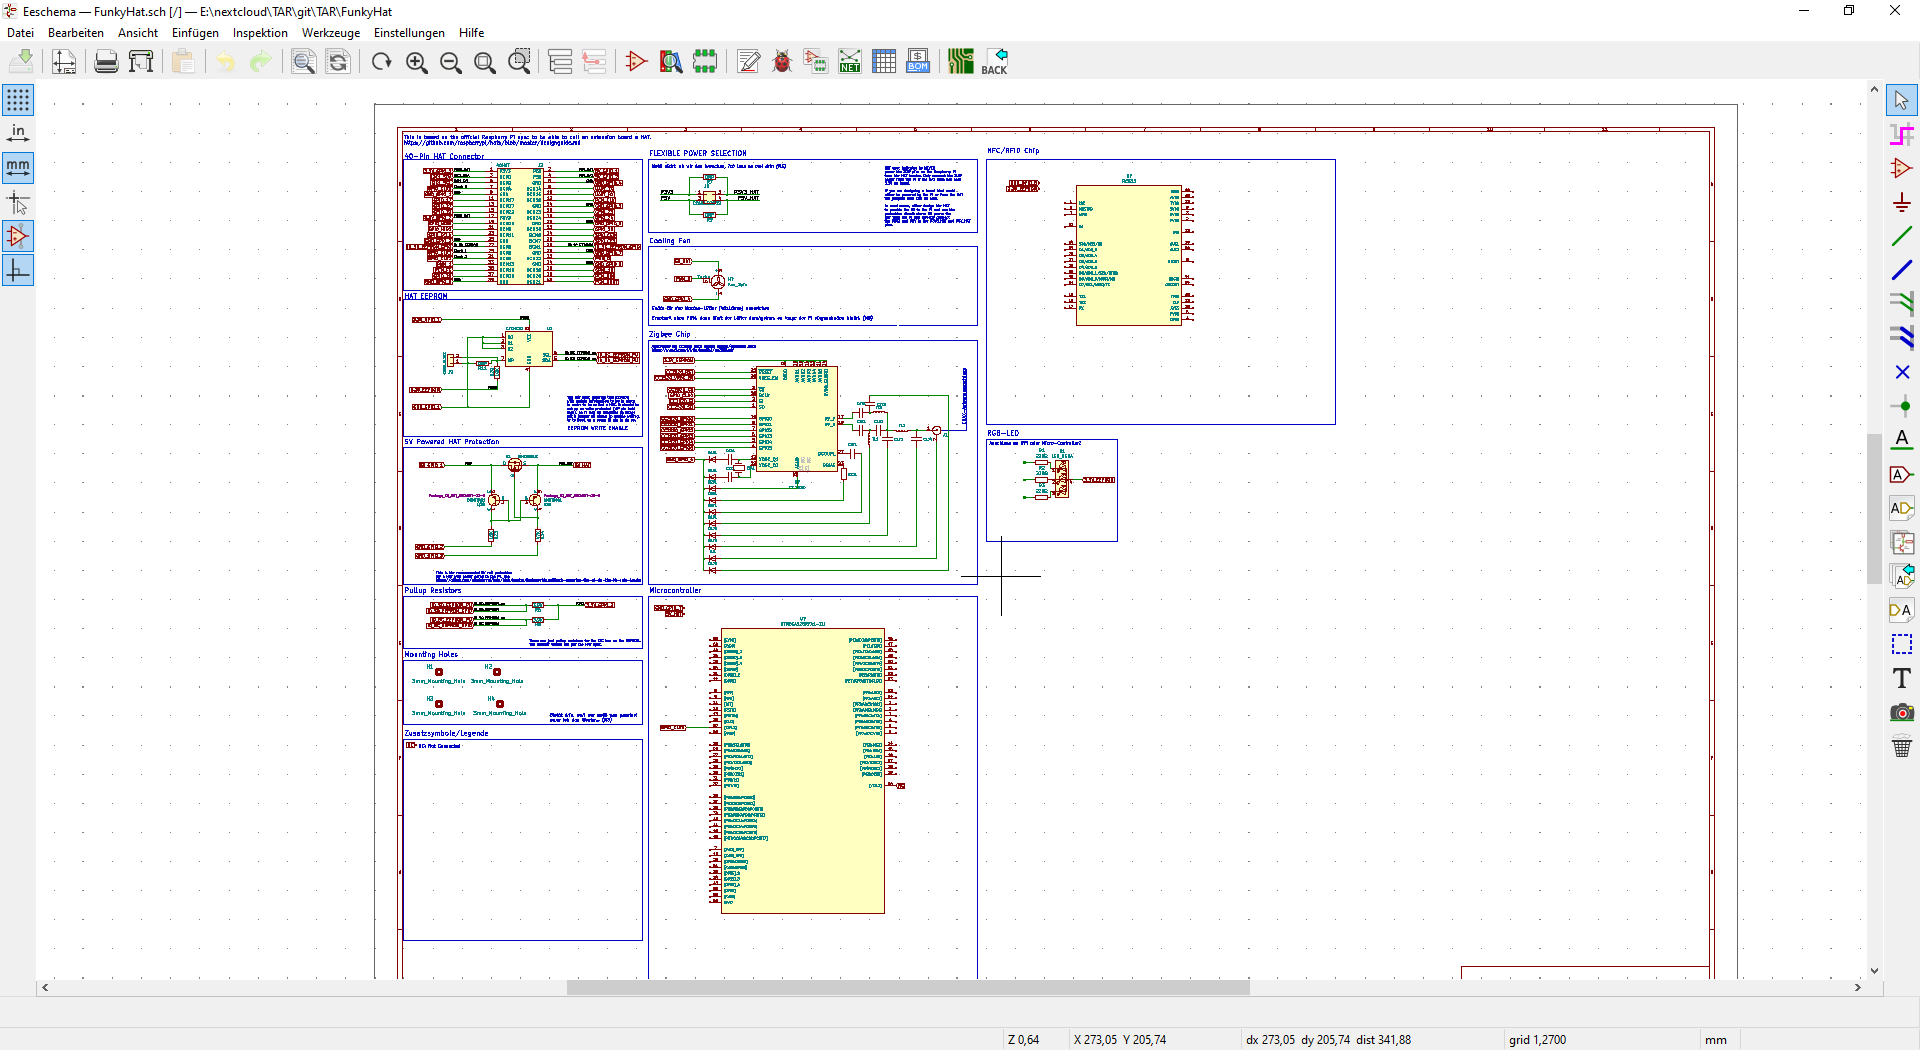
\includegraphics[width=1\textwidth]{img/stand_hat.png}
	\caption[Aktueller Stand HAT-Design]{Aktueller Stand HAT-Design}
	\label{hat-design}
\end{figure}
\noindent Aufgrund der bereits weit vorangeschrittenen Zeit im Projektplan, der aktuellen COVID-19-Pandemie und unserer Unwissenheit im Bezug auf Schaltplanentwicklung sowie der von uns verwendeten Hardware mussten wir aber einsehen, dass die Entwicklung und Fertigung eines HATs den Zeitrahmen sprengen würde und so haben wir zu Ende Februar 2021 beschlossen, dieses Projekt vorerst zurück zu stellen und uns auf die Fertistellung unserer bisherigen Testerfolge und Prototypen zu fokusieren.
Die KiCAD-Projekt-Dateien stehen, wie alle anderen Dateien des Projekts nach Abgabe frei über das entsprechende GITHUB zur Verfügung.\par